%\documentclass[12pt,letterpaper,margin=0.75in]{article}
%\documentclass[12pt]{article}

\documentclass[12pt, onecolumn]{IEEEtran}

\usepackage[utf8]{inputenc}
\usepackage{amsmath}
\usepackage{amsfonts}
\usepackage{amssymb}
\usepackage{graphicx}
\author{George Engel\\
IC Design Research Laboratory\\
Southern Illinois University Edwardsville\\
}
\usepackage{geometry}

\geometry{
 letterpaper,
% total={8.5in,11in},
 left=1.0in,
 right=1.0in,
 top=1.0in,
 bottom=1.0in,
 }

\usepackage{filecontents}
\usepackage[noadjust]{cite}

%\begin{filecontents*}{bibi.bib}
%@ARTICLE{507173,
%author={Simpson, M.L. and Young, G.R. and Jackson, R.G. and Xu, M.}, 
%journal={Nuclear Science, IEEE Transactions on}, 
%title={A monolithic, constant-fraction discriminator using distributed R-C delay line shaping}, 
%year={1996}, 
%volume={43}, 
%number={3}, 
%pages={1695-1699}, 
%keywords={CMOS logic circuits;RC circuits;delay lines;detector circuits;discriminators;monolithic integrated circuits;nuclear electronics;20 mV to 2 V;N-well process;constant-fraction shaping;delay line;distributed R-C delay line shaping;monolithic CMOS constant-fraction discriminator;monolithic constant-fraction discriminator;slope degradation;timing errors;CMOS process;Capacitors;Circuits;Computational fluid dynamics;Delay lines;Detectors;Feedback;Laboratories;Signal generators;Timing}, 
%doi={10.1109/23.507173}, 
%ISSN={0018-9499}, 
%month={Jun},} 
%\end{filecontents*}

\title{Zero-Cross Detector Design Report}

\begin{document}

% Insert title

\maketitle

% INTRODUCTION

\section*{Introduction}
The input to the Nowlin circuit is a an exponential unipolar pulse with amplitude, $A$, and risetime constant, $\tau_r$.  The signal associated with the differential output from the Nowlin circuit, however, is a bipolar pulse centered around analog signal ground (or what we will call AGND).  The time at which the pulse crosses through zero is independent of pulse amplitude. The zero-crossing time occurs at approximately, $t_z$. 

\begin{equation}
t_z \approx 2 \cdot \tau_r
\end{equation}

\noindent
We shall refer to the slope of this signal, when crossing through zero, as the slew rate (SR). One can show that \\

\begin{equation}
SR \approx \frac{A}{4 \cdot \tau_r}
\end{equation}

\noindent
For the minimum amplitude pulse amplitude of 15 $mV$ which the proposed chip must support, this results in a S$SR_{max}$ of 1.25 $\frac{V}{\mu s}$.\\


The purpose of the zero cross detector is to produce a digital signal marking the onset of the analog input pulse. It is important that this time be independent of pulse amplitude, $A$.The zero-cross circuit is constructed by cacading N differential amplifier stages (where we have chosen N equal to 6) each possessing a very wide bandwidth, but relatively low-gain ($\approx$ 4) with the final output stage driving a very fast analog comparator.\\  

The purpose of cascading a relatively large number of high-bandwidth but low-gain stages is to force linear operation where delay is independent of amplitude.  In short, the cascaded amplifier serves as a SR enhancer.  For a first-order system, it is well-known that if the input risetime is not to be severely degraded, the bandwidth, BW, of the amplifier must obey the following equation\\

\begin{equation}
BW > \frac{0.35}{t_{10-90}} \approx \text{ 50 MHz}
\end{equation}

\noindent
In the equation above we have assumed the shortest risetime constant that we must accommodate, \emph{i.e.}  3 $ns$. Since we are cascading N stages, the BW of each stage must be increased by $\sqrt{N} \approx 2.5$ resulting in a differential amplifier bandwidth of 125 MHz if the overall BW is to be 50 MHz.  If the stage gain, G, is 4 then the GBW of a single differential amplifier stage needs to be around 500 MHz. \\



\section*{Design of Zero-Cross Differential Amplifier}
We will now describe the design of the wide-bandwidth, low-gain differential amplifier described above and shown in Figure~\ref{FIG:ZC_DM_AMP}. 

\begin{figure}[htbp!]
	\centering
 	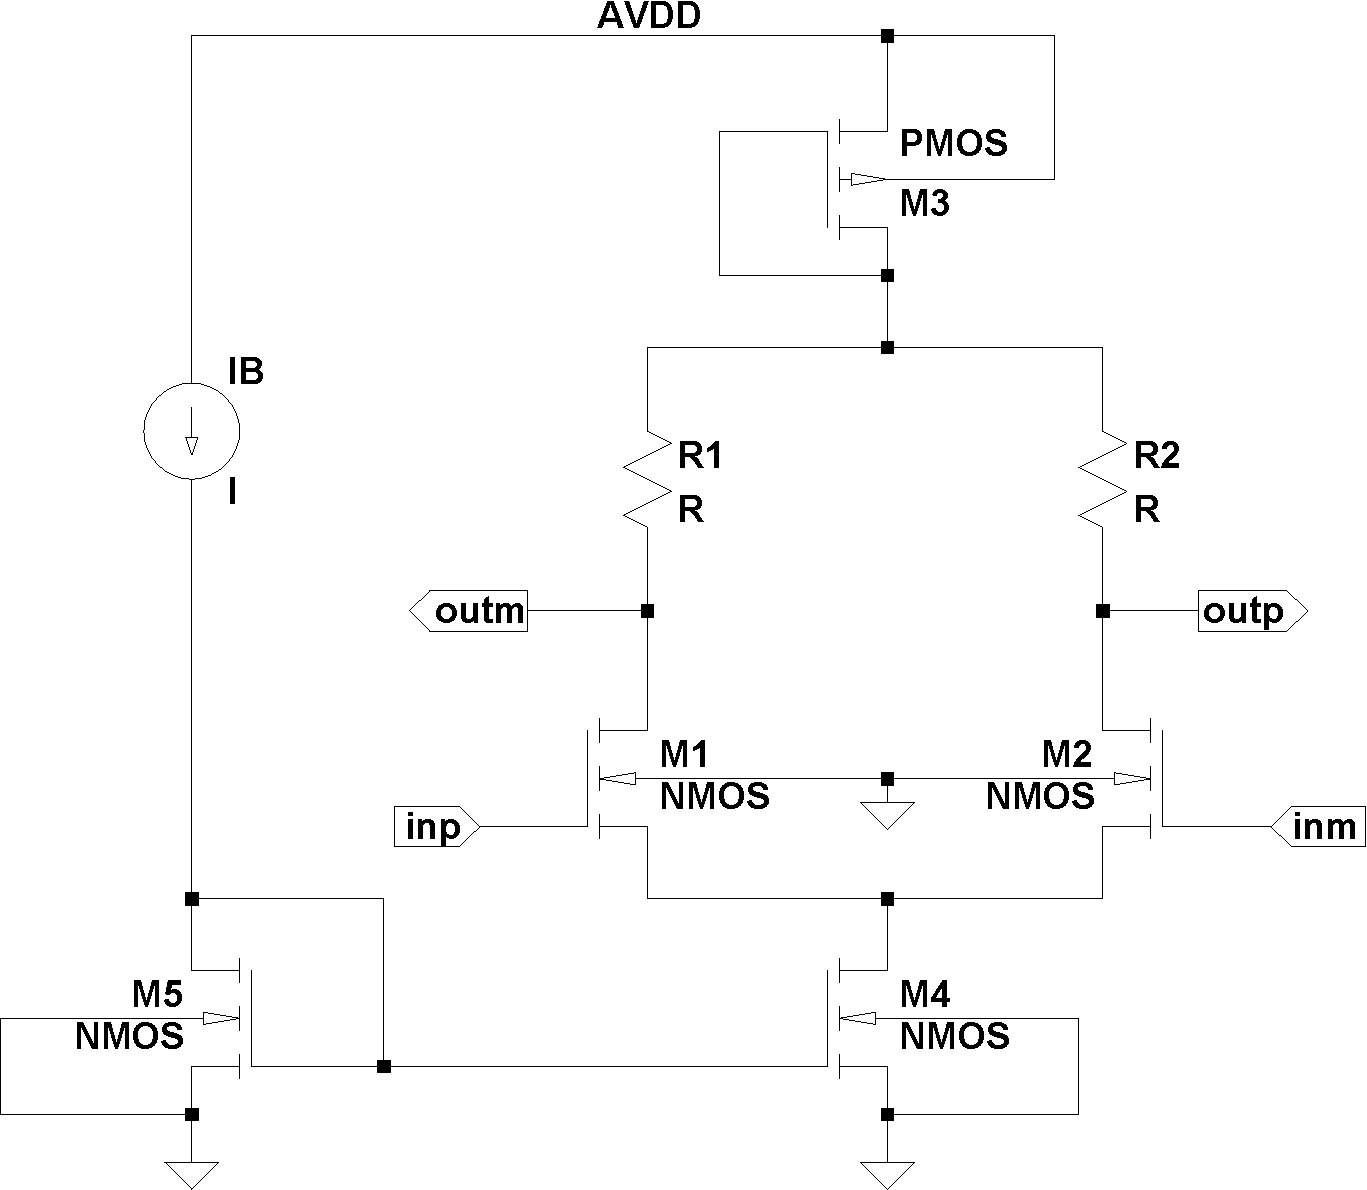
\includegraphics[scale=0.4,keepaspectratio=true]{./images/zc_dm_amp.pdf}
 	\caption{Schematic of low-gain high-bandwidth differential amplfier.}
 	\label{FIG:ZC_DM_AMP}
\end{figure}
 
 
Device sizes and bias currents are given in Table~\ref{TBL:ZC_DM_AMP}.\\ 
\begin{table} [htbp!]
\begin{center}
\begin{tabular}{|c|c|c|c|c|}
\hline 
• & Width $\mu m$ & Length $\mu m$ &  Multiplier & Bias $\mu A$ \\ 
\hline 
M1 & 1.4 & 0.35 & 1 & • \\ 
\hline 
M2 & 1.4 & 0.35 & 1 & • \\ 
\hline 
M3 & 6.8 & 0.7 & 1 & • \\ 
\hline 
M4 & 6.8 & 0.7 & 1 & • \\ 
\hline 
M5 & 1.0 & 0.35 & 1 & N/A \\ 
\hline 
M6 & 2.8 & 0.35 & 1 & N/A \\ 
\hline 
M7 & 3.0 & 0.35 & 1 & N/A \\ 
\hline 
M8 & 8.4 & 0.35 & 1 & N/A \\ 
\hline 
\end{tabular} 
\end{center}
\label{TBL:ZC_DM_AMP}
\caption{Device Sizes for Zero-Cross Detector Differential Amplifier}
\end{table}

\section*{Design of Zero-Cross Common Mode Amplifier}


\end{document}